\PassOptionsToPackage{unicode=true}{hyperref} % options for packages loaded elsewhere
\PassOptionsToPackage{hyphens}{url}
%
\documentclass[ignorenonframetext,]{beamer}
\usepackage{pgfpages}
\setbeamertemplate{caption}[numbered]
\setbeamertemplate{caption label separator}{: }
\setbeamercolor{caption name}{fg=normal text.fg}
\beamertemplatenavigationsymbolsempty
% Prevent slide breaks in the middle of a paragraph:
\widowpenalties 1 10000
\raggedbottom
\setbeamertemplate{part page}{
\centering
\begin{beamercolorbox}[sep=16pt,center]{part title}
  \usebeamerfont{part title}\insertpart\par
\end{beamercolorbox}
}
\setbeamertemplate{section page}{
\centering
\begin{beamercolorbox}[sep=12pt,center]{part title}
  \usebeamerfont{section title}\insertsection\par
\end{beamercolorbox}
}
\setbeamertemplate{subsection page}{
\centering
\begin{beamercolorbox}[sep=8pt,center]{part title}
  \usebeamerfont{subsection title}\insertsubsection\par
\end{beamercolorbox}
}
\AtBeginPart{
  \frame{\partpage}
}
\AtBeginSection{
  \ifbibliography
  \else
    \frame{\sectionpage}
  \fi
}
\AtBeginSubsection{
  \frame{\subsectionpage}
}
\usepackage{lmodern}
\usepackage{amssymb,amsmath}
\usepackage{ifxetex,ifluatex}
\usepackage{fixltx2e} % provides \textsubscript
\ifnum 0\ifxetex 1\fi\ifluatex 1\fi=0 % if pdftex
  \usepackage[T1]{fontenc}
  \usepackage[utf8]{inputenc}
  \usepackage{textcomp} % provides euro and other symbols
\else % if luatex or xelatex
  \usepackage{unicode-math}
  \defaultfontfeatures{Ligatures=TeX,Scale=MatchLowercase}
\fi
% use upquote if available, for straight quotes in verbatim environments
\IfFileExists{upquote.sty}{\usepackage{upquote}}{}
% use microtype if available
\IfFileExists{microtype.sty}{%
\usepackage[]{microtype}
\UseMicrotypeSet[protrusion]{basicmath} % disable protrusion for tt fonts
}{}
\IfFileExists{parskip.sty}{%
\usepackage{parskip}
}{% else
\setlength{\parindent}{0pt}
\setlength{\parskip}{6pt plus 2pt minus 1pt}
}
\usepackage{hyperref}
\hypersetup{
            pdftitle={Model selection, cross validation, and performance of time series models},
            pdfauthor={Eric Ward, warde@uw.edu},
            pdfborder={0 0 0},
            breaklinks=true}
\urlstyle{same}  % don't use monospace font for urls
\newif\ifbibliography
\usepackage{color}
\usepackage{fancyvrb}
\newcommand{\VerbBar}{|}
\newcommand{\VERB}{\Verb[commandchars=\\\{\}]}
\DefineVerbatimEnvironment{Highlighting}{Verbatim}{commandchars=\\\{\}}
% Add ',fontsize=\small' for more characters per line
\usepackage{framed}
\definecolor{shadecolor}{RGB}{248,248,248}
\newenvironment{Shaded}{\begin{snugshade}}{\end{snugshade}}
\newcommand{\AlertTok}[1]{\textcolor[rgb]{0.94,0.16,0.16}{#1}}
\newcommand{\AnnotationTok}[1]{\textcolor[rgb]{0.56,0.35,0.01}{\textbf{\textit{#1}}}}
\newcommand{\AttributeTok}[1]{\textcolor[rgb]{0.77,0.63,0.00}{#1}}
\newcommand{\BaseNTok}[1]{\textcolor[rgb]{0.00,0.00,0.81}{#1}}
\newcommand{\BuiltInTok}[1]{#1}
\newcommand{\CharTok}[1]{\textcolor[rgb]{0.31,0.60,0.02}{#1}}
\newcommand{\CommentTok}[1]{\textcolor[rgb]{0.56,0.35,0.01}{\textit{#1}}}
\newcommand{\CommentVarTok}[1]{\textcolor[rgb]{0.56,0.35,0.01}{\textbf{\textit{#1}}}}
\newcommand{\ConstantTok}[1]{\textcolor[rgb]{0.00,0.00,0.00}{#1}}
\newcommand{\ControlFlowTok}[1]{\textcolor[rgb]{0.13,0.29,0.53}{\textbf{#1}}}
\newcommand{\DataTypeTok}[1]{\textcolor[rgb]{0.13,0.29,0.53}{#1}}
\newcommand{\DecValTok}[1]{\textcolor[rgb]{0.00,0.00,0.81}{#1}}
\newcommand{\DocumentationTok}[1]{\textcolor[rgb]{0.56,0.35,0.01}{\textbf{\textit{#1}}}}
\newcommand{\ErrorTok}[1]{\textcolor[rgb]{0.64,0.00,0.00}{\textbf{#1}}}
\newcommand{\ExtensionTok}[1]{#1}
\newcommand{\FloatTok}[1]{\textcolor[rgb]{0.00,0.00,0.81}{#1}}
\newcommand{\FunctionTok}[1]{\textcolor[rgb]{0.00,0.00,0.00}{#1}}
\newcommand{\ImportTok}[1]{#1}
\newcommand{\InformationTok}[1]{\textcolor[rgb]{0.56,0.35,0.01}{\textbf{\textit{#1}}}}
\newcommand{\KeywordTok}[1]{\textcolor[rgb]{0.13,0.29,0.53}{\textbf{#1}}}
\newcommand{\NormalTok}[1]{#1}
\newcommand{\OperatorTok}[1]{\textcolor[rgb]{0.81,0.36,0.00}{\textbf{#1}}}
\newcommand{\OtherTok}[1]{\textcolor[rgb]{0.56,0.35,0.01}{#1}}
\newcommand{\PreprocessorTok}[1]{\textcolor[rgb]{0.56,0.35,0.01}{\textit{#1}}}
\newcommand{\RegionMarkerTok}[1]{#1}
\newcommand{\SpecialCharTok}[1]{\textcolor[rgb]{0.00,0.00,0.00}{#1}}
\newcommand{\SpecialStringTok}[1]{\textcolor[rgb]{0.31,0.60,0.02}{#1}}
\newcommand{\StringTok}[1]{\textcolor[rgb]{0.31,0.60,0.02}{#1}}
\newcommand{\VariableTok}[1]{\textcolor[rgb]{0.00,0.00,0.00}{#1}}
\newcommand{\VerbatimStringTok}[1]{\textcolor[rgb]{0.31,0.60,0.02}{#1}}
\newcommand{\WarningTok}[1]{\textcolor[rgb]{0.56,0.35,0.01}{\textbf{\textit{#1}}}}
\usepackage{graphicx,grffile}
\makeatletter
\def\maxwidth{\ifdim\Gin@nat@width>\linewidth\linewidth\else\Gin@nat@width\fi}
\def\maxheight{\ifdim\Gin@nat@height>\textheight\textheight\else\Gin@nat@height\fi}
\makeatother
% Scale images if necessary, so that they will not overflow the page
% margins by default, and it is still possible to overwrite the defaults
% using explicit options in \includegraphics[width, height, ...]{}
\setkeys{Gin}{width=\maxwidth,height=\maxheight,keepaspectratio}
\setlength{\emergencystretch}{3em}  % prevent overfull lines
\providecommand{\tightlist}{%
  \setlength{\itemsep}{0pt}\setlength{\parskip}{0pt}}
\setcounter{secnumdepth}{0}

% set default figure placement to htbp
\makeatletter
\def\fps@figure{htbp}
\makeatother


\title{Model selection, cross validation, and performance of time series models}
\providecommand{\subtitle}[1]{}
\subtitle{FISH 507 -- Applied Time Series Analysis}
\author{Eric Ward, \href{mailto:warde@uw.edu}{\nolinkurl{warde@uw.edu}}}
\date{January 29 2019}

\begin{document}
\frame{\titlepage}

\begin{frame}[fragile]

\begin{block}{Overview of today's material}

\begin{itemize}
\tightlist
\item
  Approaches for model selection
\item
  Cross validation
\item
  Quantifying forecast performance
\end{itemize}

\end{block}

\begin{block}{How good are our models?}

Several candidate models might be built based on

\begin{itemize}
\tightlist
\item
  hypotheses / mechanisms
\item
  diagnostics / summaries of fit
\end{itemize}

Models can be evaluated by their ability to explain data

\begin{itemize}
\tightlist
\item
  OR by the tradeoff in the ability to explain data, and ability to
  predict future data
\item
  OR just in their predictive abilities

  \begin{itemize}
  \tightlist
  \item
    Hindcasting
  \item
    Forecasting
  \end{itemize}
\end{itemize}

\end{block}

\begin{block}{How good are our models?}

We can illustrate with an example to the \texttt{harborSealWA} dataset
in MARSS

\begin{center}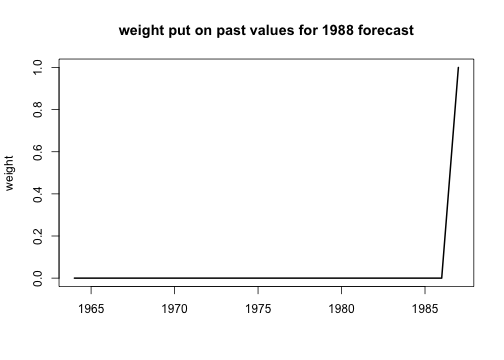
\includegraphics{lec_7_modelselection_files/figure-beamer/unnamed-chunk-1-1} \end{center}

\end{block}

\begin{block}{How good are our models?}

Metrics like the sum of squares are appealing,

\[SS=\sum _{ i=1 }^{ n }{ { \left( y_{ i }-E[{ y }_{ i }] \right)  }^{ 2 } } \]

\end{block}

\begin{block}{How good are our models?}

\begin{verbatim}
## 
## Call:
## lm(formula = SJI ~ Year, data = harborSealWA)
## 
## Residuals:
##      Min       1Q   Median       3Q      Max 
## -0.46099 -0.08022  0.06576  0.13286  0.21464 
## 
## Coefficients:
##               Estimate Std. Error t value Pr(>|t|)    
## (Intercept) -1.392e+02  1.601e+01  -8.697 1.85e-07 ***
## Year         7.397e-02  8.043e-03   9.197 8.69e-08 ***
## ---
## Signif. codes:  0 '***' 0.001 '**' 0.01 '*' 0.05 '.' 0.1 ' ' 1
## 
## Residual standard error: 0.1916 on 16 degrees of freedom
##   (4 observations deleted due to missingness)
## Multiple R-squared:  0.8409, Adjusted R-squared:  0.831 
## F-statistic: 84.58 on 1 and 16 DF,  p-value: 8.693e-08
\end{verbatim}

\end{block}

\begin{block}{How good are our models?}

Our regression model had a pretty good sum-of-squares

\begin{itemize}
\tightlist
\item
  But SS is problematic

  \begin{itemize}
  \tightlist
  \item
    as we consider more complex models, they'll inevitably reduce SS
  \item
    there's no cost or penalty for having too many parameters
  \end{itemize}
\end{itemize}

\end{block}

\begin{block}{Model selection}

Lots of metrics have been developed to overcome this issue and penalize
complex models

\begin{itemize}
\item
  \textbf{Occam's razor}: ``the law of briefness''
\item
  \textbf{Principle of parsimony}: choose the simplest possible model
  that explains the data pretty well

  \begin{itemize}
  \tightlist
  \item
    choose a model that minimizes bias \emph{and} variance
  \end{itemize}
\end{itemize}

\end{block}

\begin{block}{Model selection}

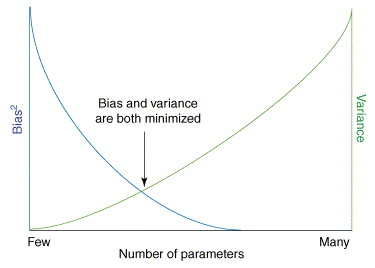
\includegraphics{https://www.cell.com/cms/attachment/586583/4453621/gr1b1.jpg}
\url{https://doi.org/10.1016/j.tree.2006.10.004}

\end{block}

\begin{block}{Model selection: AIC}

Akaike's Information Criterion (\textbf{AIC}, Akaike 1973)

\begin{itemize}
\item
  Attempts to balance the goodness of fit of the model against the
  number of parameters
\item
  Based on deviance = minus twice negative log likelihood
\end{itemize}

Deviance =
\[-2\cdot ln\left( L(\underline { \theta } |\underline { y  } ) \right)\]

\begin{itemize}
\tightlist
\item
  Deviance is a measure of model fit to data

  \begin{itemize}
  \tightlist
  \item
    lower values are better
  \item
    Maximizing likelihood is equivalent to minimizing negative
    likelihood
  \end{itemize}
\end{itemize}

\end{block}

\begin{block}{Model selection: AIC}

Many *IC approaches to model selection also rely on deviance. Where they
differ is how they structure the penalty term.

For AIC, the penalty is 2 * number of parameters (\(k\)),

\[AIC = -2\cdot ln\left( L(\underline { \theta } |\underline { y  } ) \right) + 2k\]

\begin{itemize}
\tightlist
\item
  But what about sample size, \(n\)?
\end{itemize}

\end{block}

\begin{block}{Model selection: AIC}

Small sample AIC

\[AICc=AIC+\frac { 2k(k+1) }{ n-k-1 }\]

\begin{itemize}
\tightlist
\item
  What happens to this term as n increases?
\end{itemize}

\end{block}

\begin{block}{Model selection: AIC}

AIC aims to find the best model to predict data generated from the same
process that generated your observations

Downside: AIC has a tendency to overpenalize, especially for more
complex models

\begin{itemize}
\tightlist
\item
  Equivalent to significance test w/ \(\alpha\) = 0.16
\end{itemize}

Alternative: Schwarz/Bayesian Information Criterion (SIC/BIC)

\begin{itemize}
\tightlist
\item
  Not Bayesian!
\item
  Relies on Laplace approximation to posterior
\item
  \(\alpha\) becomes a function of sample size
\end{itemize}

\end{block}

\begin{block}{Model selection: AIC}

BIC is measure of explanatory power (rather than balancing explanation /
prediction)

\[BIC = -2\cdot ln\left( L(\underline { \theta } |\underline { y  } ) \right) + k\cdot ln(n)\]

\begin{itemize}
\tightlist
\item
  Tendency of BIC to underpenalize
\end{itemize}

\end{block}

\begin{block}{Model selection: AIC}

Philosophical differences between AIC / BIC

\begin{itemize}
\tightlist
\item
  AIC / AICc tries to choose a model that approximates reality

  \begin{itemize}
  \tightlist
  \item
    does not assume that reality exists in your set of candidate models
  \end{itemize}
\item
  BIC assumes that one of your models is truth

  \begin{itemize}
  \tightlist
  \item
    This model will tend to be favored more as sample size increases
  \end{itemize}
\end{itemize}

\end{block}

\begin{block}{Model selection: AIC}

Many base functions in R support the extraction of AIC

\begin{Shaded}
\begin{Highlighting}[]
\NormalTok{y =}\StringTok{ }\KeywordTok{cumsum}\NormalTok{(}\KeywordTok{rnorm}\NormalTok{(}\DecValTok{20}\NormalTok{))}
\KeywordTok{AIC}\NormalTok{(}\KeywordTok{lm}\NormalTok{(y}\OperatorTok{~}\DecValTok{1}\NormalTok{))}
\KeywordTok{AIC}\NormalTok{(}\KeywordTok{glm}\NormalTok{(y}\OperatorTok{~}\DecValTok{1}\NormalTok{))}
\KeywordTok{AIC}\NormalTok{(mgcv}\OperatorTok{::}\KeywordTok{gam}\NormalTok{(y}\OperatorTok{~}\DecValTok{1}\NormalTok{))}
\KeywordTok{AIC}\NormalTok{(glmmTMB}\OperatorTok{::}\KeywordTok{glmmTMB}\NormalTok{(y}\OperatorTok{~}\DecValTok{1}\NormalTok{))}
\KeywordTok{AIC}\NormalTok{(lme4}\OperatorTok{::}\KeywordTok{lmer}\NormalTok{(y}\OperatorTok{~}\DecValTok{1}\NormalTok{))}
\KeywordTok{AIC}\NormalTok{(stats}\OperatorTok{::}\KeywordTok{arima}\NormalTok{(y))}
\KeywordTok{AIC}\NormalTok{(forecast}\OperatorTok{::}\KeywordTok{Arima}\NormalTok{(y))}
\end{Highlighting}
\end{Shaded}

\end{block}

\begin{block}{Bayesian model selection}

Largely beyond the scope of this class, but as an overview there's
several options

\begin{itemize}
\tightlist
\item
  Bayes factors (approximated by BIC)

  \begin{itemize}
  \tightlist
  \item
    can be very difficult to calculate for complex models
  \end{itemize}
\item
  Deviance Information Criterion (DIC)

  \begin{itemize}
  \tightlist
  \item
    Spiegelhalter et al.~(2002)
  \item
    DIC is easy to get out of some programs (JAGS)
  \end{itemize}
\end{itemize}

DIC is also attempting to balance bias and variance

\end{block}

\begin{block}{Bayesian model selection}

Like AIC, DIC is estimated from (1) the deviance, and (2) penalty, or
effective number of parameters \(p_{D}\).
\[DIC = -2\cdot ln\left( L(\underline { \theta } |\underline { y  } ) \right) + 2p_{D}\]
Options for \(p_{D}\) are

\begin{itemize}
\item
  \(E[D]-D\left( \bar { \theta } \right)\) (Spiegelhalter et al.~2002)
  and
\item
  \(\frac { Var(D\left( \theta \right) ) }{ 2 }\) (Gelman et al.~2004)
\end{itemize}

\end{block}

\begin{block}{Bayesian model selection}

The big difference between the Bayesian and maximum likelihood
approaches are that

\begin{itemize}
\tightlist
\item
  ML methods are maximizing the likelihood over the parameter space
\item
  Bayesian methods are integrating over the parameter space, asking
  `what values are best, on average?'
\end{itemize}

Many of the ML methods discussed were designed for models with only
fixed effects.

\begin{itemize}
\tightlist
\item
  What about correlated parameters, nested or hierarchical models?
\end{itemize}

\end{block}

\begin{block}{Cross validation}

Recent focus in ecology \& fisheries on prediction

\href{https://esajournals.onlinelibrary.wiley.com/doi/full/10.1002/eap.1589}{Dietze
et al.~2017}

\href{https://onlinelibrary.wiley.com/doi/full/10.1111/oik.04655}{Maris
et al.~2017}

\href{https://www.sciencedirect.com/science/article/pii/S1476945X16301106}{Pennekamp
et al.~2017}

\href{https://www.biorxiv.org/content/early/2018/06/19/350017}{Pennekamp
et al.~2018}

\href{https://onlinelibrary.wiley.com/doi/abs/10.1111/faf.12226}{Szuwalkski
\& Thorson 2017}

\href{https://onlinelibrary.wiley.com/doi/abs/10.1111/faf.12200}{Anderson
et al.~2017}

\end{block}

\begin{block}{Resampling techniques}

\textbf{Jackknife}

\begin{itemize}
\tightlist
\item
  Hold out each data point, recomputing some statistic (and then average
  across 1:n)
\end{itemize}

\textbf{Bootstrap}

\begin{itemize}
\tightlist
\item
  Similar to jackknife, but with resampling
\end{itemize}

\textbf{Cross-validation (k-fold)}

\begin{itemize}
\tightlist
\item
  Divide dataset into k-partitions
\item
  How well do (k-1) partitions predict kth set of points?
\item
  Relationship between LOOCV and AIC
\end{itemize}

\textbf{Data split}: test/training sets (e.g.~holdout last 5 data pts)

\end{block}

\begin{block}{Resampling techniques}

Bootstrap or jackknife approaches are useful

\begin{itemize}
\item
  generally used in the context of time series models to generate new or
  pseudo-datasets
\item
  state space models: use estimated deviations / errors to simulate,
  estimate CIs
\end{itemize}

Examples

\begin{Shaded}
\begin{Highlighting}[]
\NormalTok{MARSS}\OperatorTok{::}\KeywordTok{MARSSboot}\NormalTok{()}
\NormalTok{MARSS}\OperatorTok{::}\KeywordTok{MARSSinnovationsboot}\NormalTok{()}
\NormalTok{forecast}\OperatorTok{::}\KeywordTok{bld.mbb.bootstrap}\NormalTok{()}
\NormalTok{forecast}\OperatorTok{::}\KeywordTok{forecast}\NormalTok{(..., }\DataTypeTok{bootstrap=}\OtherTok{TRUE}\NormalTok{)}
\end{Highlighting}
\end{Shaded}

\end{block}

\begin{block}{Resampling techniques}

As an example, we'll use a time series of body temperature from the
\texttt{beavers} dataset

\begin{Shaded}
\begin{Highlighting}[]
\KeywordTok{data}\NormalTok{(beavers)}
\NormalTok{beaver =}\StringTok{ }\NormalTok{dplyr}\OperatorTok{::}\KeywordTok{filter}\NormalTok{(beaver2, time}\OperatorTok{>}\DecValTok{200}\NormalTok{)}
\end{Highlighting}
\end{Shaded}

\begin{Shaded}
\begin{Highlighting}[]
\KeywordTok{ggplot}\NormalTok{(beaver, }\KeywordTok{aes}\NormalTok{(time, temp)) }\OperatorTok{+}\StringTok{ }
\StringTok{  }\KeywordTok{geom_point}\NormalTok{() }\OperatorTok{+}\StringTok{ }\KeywordTok{geom_line}\NormalTok{() }\OperatorTok{+}\StringTok{ }
\StringTok{  }\KeywordTok{ylab}\NormalTok{(}\StringTok{"Temperature"}\NormalTok{) }\OperatorTok{+}\StringTok{ }\KeywordTok{xlab}\NormalTok{(}\StringTok{"Time"}\NormalTok{)}
\end{Highlighting}
\end{Shaded}

\begin{center}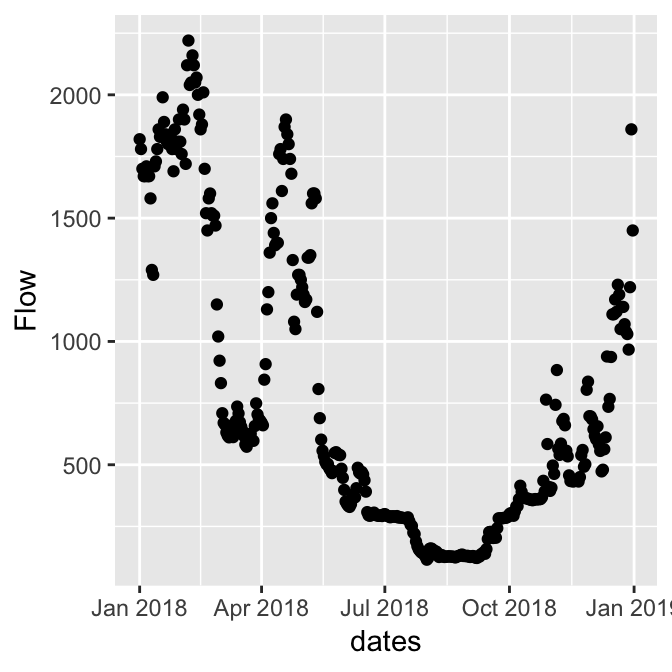
\includegraphics{lec_7_modelselection_files/figure-beamer/unnamed-chunk-6-1} \end{center}

\end{block}

\begin{block}{Resampling techniques: K-fold cross validation}

\begin{itemize}
\tightlist
\item
  Choose model (e.g.~regression)
\item
  Partition data
\item
  Fit \& prediction
\end{itemize}

Things to highlight: \# folds, how sampling is done

\begin{Shaded}
\begin{Highlighting}[]
\NormalTok{K =}\StringTok{ }\DecValTok{5} 
\NormalTok{beaver}\OperatorTok{$}\NormalTok{part =}\StringTok{ }\KeywordTok{sample}\NormalTok{(}\DecValTok{1}\OperatorTok{:}\NormalTok{K, }\DataTypeTok{size=}\KeywordTok{nrow}\NormalTok{(beaver), }\DataTypeTok{replace=}\NormalTok{T)}
\NormalTok{beaver}\OperatorTok{$}\NormalTok{pred =}\StringTok{ }\DecValTok{0}
\ControlFlowTok{for}\NormalTok{(i }\ControlFlowTok{in} \DecValTok{1}\OperatorTok{:}\NormalTok{K) \{}
\NormalTok{    mod =}\StringTok{ }\KeywordTok{lm}\NormalTok{(temp}\OperatorTok{~}\NormalTok{time, }\DataTypeTok{data =}\NormalTok{ beaver[beaver}\OperatorTok{$}\NormalTok{part}\OperatorTok{!=}\NormalTok{i,])}
\NormalTok{    beaver}\OperatorTok{$}\NormalTok{pred[beaver}\OperatorTok{$}\NormalTok{part}\OperatorTok{==}\NormalTok{i] =}\StringTok{ }
\StringTok{    }\KeywordTok{predict}\NormalTok{(mod, }\DataTypeTok{newdata =}\NormalTok{ beaver[beaver}\OperatorTok{$}\NormalTok{part}\OperatorTok{==}\NormalTok{i,])}
\NormalTok{\}}
\end{Highlighting}
\end{Shaded}

\end{block}

\begin{block}{Resampling techniques: K-fold cross validation}

\begin{center}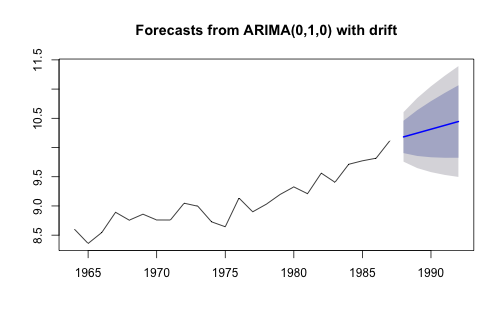
\includegraphics{lec_7_modelselection_files/figure-beamer/unnamed-chunk-8-1} \end{center}

\end{block}

\begin{block}{Resampling techniques: K-fold cross validation}

\begin{itemize}
\item
  How large should K be?
\item
  Bias/variance tradeoff:
\item
  Low K: low variance, larger bias, quicker to run. ML approaches
  recommend 5-10
\item
  High K (LOOCV): low bias, high variance, computationally expensive
\end{itemize}

\end{block}

\begin{block}{Resampling techniques: repeated K-fold cross validation}

\begin{itemize}
\item
  To remove effect of random sampling / partitioning, repeat K-fold
  cross validation and average predictions for a given data point
\item
  caret() package in R
\end{itemize}

\end{block}

\begin{block}{Resampling techniques: repeated K-fold cross validation}

\begin{itemize}
\tightlist
\item
  Need to specify repeats
\end{itemize}

\begin{Shaded}
\begin{Highlighting}[]
\NormalTok{train_control =}\StringTok{ }\NormalTok{caret}\OperatorTok{::}\KeywordTok{trainControl}\NormalTok{(}\DataTypeTok{method=}\StringTok{"repeatedcv"}\NormalTok{, }
                \DataTypeTok{number=}\DecValTok{5}\NormalTok{, }\DataTypeTok{repeats=}\DecValTok{20}\NormalTok{)}
\end{Highlighting}
\end{Shaded}

\begin{itemize}
\tightlist
\item
  Again this is extendable across many widely used models
\end{itemize}

\end{block}

\begin{block}{Resampling techniques: repeated K-fold cross validation}

\begin{Shaded}
\begin{Highlighting}[]
\KeywordTok{summary}\NormalTok{(model)}
\end{Highlighting}
\end{Shaded}

Call: lm(formula = .outcome \textasciitilde{} ., data = dat)

Residuals: Min 1Q Median 3Q Max -0.5553 -0.2160 -0.1019 0.2139 0.6868

Coefficients: Estimate Std. Error t value
Pr(\textgreater{}\textbar{}t\textbar{})\\
(Intercept) 3.613e+01 1.266e-01 285.30 \textless{}2e-16 \textbf{\emph{
time 8.795e-04 7.441e-05 11.82 \textless{}2e-16 }} --- Signif. codes: 0
`\emph{\textbf{' 0.001 '}' 0.01 '}' 0.05 `.' 0.1 ' ' 1

Residual standard error: 0.2905 on 85 degrees of freedom Multiple
R-squared: 0.6218, Adjusted R-squared: 0.6173 F-statistic: 139.7 on 1
and 85 DF, p-value: \textless{} 2.2e-16

\end{block}

\begin{block}{Resampling techniques}

What about for time series data?

\begin{itemize}
\tightlist
\item
  Previous resampling was random
\item
  No preservation of order (autocorrelation)
\end{itemize}

\end{block}

\begin{block}{Resampling techniques: forward chain CV}

Idea: only evaluate models on subsequent data

\begin{itemize}
\tightlist
\item
  Fold 1: training{[}1{]}, test{[}2{]}
\item
  Fold 2: training{[}1:2{]}, test{[}3{]}
\item
  Fold 3: training{[}1:3{]}, test{[}4{]}
\item
  Fold 4: training{[}1:4{]}, test{[}5{]}
\end{itemize}

\end{block}

\begin{block}{Resampling techniques: forward chain CV}

Example with Arima(1,1,1) model

\begin{itemize}
\tightlist
\item
  Assign partitions in order, 1:5
\end{itemize}

\begin{Shaded}
\begin{Highlighting}[]
\NormalTok{beaver}\OperatorTok{$}\NormalTok{part =}\StringTok{ }\KeywordTok{ceiling}\NormalTok{(}\DecValTok{5}\OperatorTok{*}\KeywordTok{seq}\NormalTok{(}\DecValTok{1}\NormalTok{,}\KeywordTok{nrow}\NormalTok{(beaver)) }\OperatorTok{/}\StringTok{ }\NormalTok{(}\KeywordTok{nrow}\NormalTok{(beaver)))}
\end{Highlighting}
\end{Shaded}

\begin{itemize}
\tightlist
\item
  iterate through 2:5 fitting the model and forecasting
\end{itemize}

\end{block}

\begin{block}{Resampling techniques: forward chain CV}

Example code:

\begin{Shaded}
\begin{Highlighting}[]
\ControlFlowTok{for}\NormalTok{(i }\ControlFlowTok{in} \DecValTok{2}\OperatorTok{:}\DecValTok{5}\NormalTok{) \{}
\NormalTok{mod =}\StringTok{ }\KeywordTok{Arima}\NormalTok{(beaver}\OperatorTok{$}\NormalTok{temp[}\KeywordTok{which}\NormalTok{(beaver}\OperatorTok{$}\NormalTok{part }\OperatorTok{<}\StringTok{ }\NormalTok{i)], }\DataTypeTok{order=}\KeywordTok{c}\NormalTok{(}\DecValTok{1}\NormalTok{,}\DecValTok{1}\NormalTok{,}\DecValTok{1}\NormalTok{))}

\NormalTok{beaver}\OperatorTok{$}\NormalTok{pred[}\KeywordTok{which}\NormalTok{(beaver}\OperatorTok{$}\NormalTok{part }\OperatorTok{==}\StringTok{ }\NormalTok{i)] =}\StringTok{ }
\StringTok{  }\KeywordTok{as.numeric}\NormalTok{(}\KeywordTok{forecast}\NormalTok{(mod, }\DataTypeTok{h =} \KeywordTok{length}\NormalTok{(}\KeywordTok{which}\NormalTok{(beaver}\OperatorTok{$}\NormalTok{part }\OperatorTok{==}\StringTok{ }\NormalTok{i)))}\OperatorTok{$}\NormalTok{mean)}
\NormalTok{\}}
\end{Highlighting}
\end{Shaded}

\end{block}

\begin{block}{Bayesian cross validation}

LOOCV (Leave-one out cross validation) + preferred over alternatives

WAIC (widely applicable information criterion)

\begin{itemize}
\tightlist
\item
  Both available in \texttt{loo::loo()}
\end{itemize}

Additional reading:
\url{https://cran.r-project.org/web/packages/loo/vignettes/loo2-example.html}

\end{block}

\begin{block}{Prediction and forecast evaluations}

\end{block}

\begin{block}{Forecasting with arima()}

\begin{itemize}
\item
  Let's fit an ARMA(1,1) model to the global temperature data, after 1st
  differencing to remove trend
\item
  You can use the arima() function or Arima() function -- Arima() is a
  wrapper for arima()
\end{itemize}

\begin{center}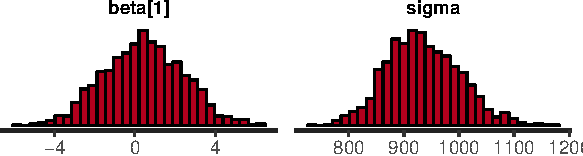
\includegraphics{lec_7_modelselection_files/figure-beamer/unnamed-chunk-14-1} \end{center}

\end{block}

\begin{block}{Forecasting with arima()}

Seasonal component not included because these data are collected
annually

\begin{Shaded}
\begin{Highlighting}[]
\NormalTok{ar.global}\FloatTok{.1}\NormalTok{ =}\StringTok{ }\KeywordTok{Arima}\NormalTok{(globtemp, }\DataTypeTok{order =} \KeywordTok{c}\NormalTok{(}\DecValTok{1}\NormalTok{,}\DecValTok{1}\NormalTok{,}\DecValTok{1}\NormalTok{),}
              \DataTypeTok{seasonal=}\KeywordTok{list}\NormalTok{(}\DataTypeTok{order=}\KeywordTok{c}\NormalTok{(}\DecValTok{0}\NormalTok{,}\DecValTok{0}\NormalTok{,}\DecValTok{0}\NormalTok{),}
              \DataTypeTok{period=}\DecValTok{12}\NormalTok{))}

\NormalTok{f1 =}\StringTok{ }\KeywordTok{forecast}\NormalTok{(ar.global}\FloatTok{.1}\NormalTok{, }\DataTypeTok{h =} \DecValTok{10}\NormalTok{)}
\end{Highlighting}
\end{Shaded}

\begin{itemize}
\tightlist
\item
  h = number of time steps to forecast in future
\end{itemize}

\end{block}

\begin{block}{Forecasting with arima()}

\begin{Shaded}
\begin{Highlighting}[]
\KeywordTok{summary}\NormalTok{(f1)}
\end{Highlighting}
\end{Shaded}

\begin{verbatim}
## 
## Forecast method: ARIMA(1,1,1)
## 
## Model Information:
## Series: globtemp 
## ARIMA(1,1,1) 
## 
## Coefficients:
##          ar1      ma1
##       0.3138  -0.6975
## s.e.  0.1400   0.0989
## 
## sigma^2 estimated as 0.01035:  log likelihood=117.81
## AIC=-229.62   AICc=-229.44   BIC=-220.91
## 
## Error measures:
##                      ME      RMSE        MAE      MPE     MAPE      MASE
## Training set 0.01578913 0.1006282 0.08541372 20.22738 76.15972 0.9569172
##                     ACF1
## Training set 0.002808596
## 
## Forecasts:
##      Point Forecast     Lo 80     Hi 80     Lo 95     Hi 95
## 2016      0.7942681 0.6638616 0.9246747 0.5948285 0.9937078
## 2017      0.7705020 0.6173184 0.9236855 0.5362279 1.0047760
## 2018      0.7630437 0.5967695 0.9293178 0.5087493 1.0173381
## 2019      0.7607031 0.5840228 0.9373834 0.4904939 1.0309123
## 2020      0.7599686 0.5739514 0.9459858 0.4754799 1.0444574
## 2021      0.7597381 0.5649751 0.9545011 0.4618738 1.0576024
## 2022      0.7596658 0.5565764 0.9627551 0.4490674 1.0702641
## 2023      0.7596431 0.5485686 0.9707176 0.4368325 1.0824537
## 2024      0.7596359 0.5408715 0.9784004 0.4250646 1.0942073
## 2025      0.7596337 0.5334418 0.9858256 0.4137030 1.1055644
\end{verbatim}

\end{block}

\begin{block}{Forecasting with arima()}

\begin{Shaded}
\begin{Highlighting}[]
\KeywordTok{plot}\NormalTok{(f1)}
\end{Highlighting}
\end{Shaded}

\begin{center}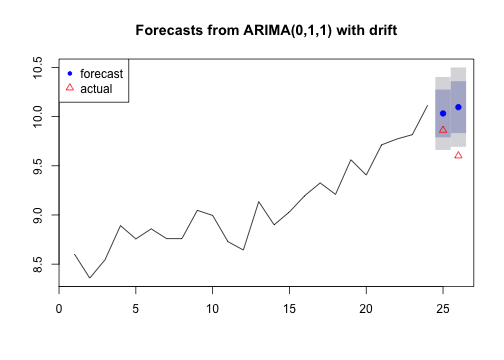
\includegraphics{lec_7_modelselection_files/figure-beamer/unnamed-chunk-17-1} \end{center}

\end{block}

\begin{block}{Quantifying forecast performance}

One of the most widelty used metrics is mean square error (MSE)

\[MSE=E\left[ { e }_{ t }^{ 2 } \right] =E\left[ { \left( { x }_{ t }-{ \hat { x }  }_{ t } \right)  }^{ 2 } \right]\]

\begin{itemize}
\tightlist
\item
  Root mean squared error (RMSE) also very common
\end{itemize}

\end{block}

\begin{block}{Quantifying forecast performance}

Like with model selection, the bias-variance tradeoff is important

\begin{itemize}
\tightlist
\item
  principle of parsimony
\end{itemize}

MSE can be rewritten as

\[MSE=Var\left( { \hat { x }  }_{ t } \right) +Bias{ \left( { x }_{ t },{ \hat { x }  }_{ t } \right)  }^{ 2 }\]
* Smaller MSE = lower bias + variance

\end{block}

\begin{block}{Quantifying forecast performance}

MSE and all forecast metrics can be calculated for

\begin{itemize}
\tightlist
\item
  single data points
\item
  entire time series
\item
  future forecasts
\end{itemize}

\[MSE={ \frac { \sum _{ t=1 }^{ n }{ { \left( { x }_{ t }-{ \hat { x }  }_{ t } \right)  }^{ 2 } }  }{ n }  }\]

\begin{itemize}
\tightlist
\item
  Do you care just about predicting the final outcome of a forecast, or
  also the trajectory to get there?
\end{itemize}

\end{block}

\begin{block}{Variants of MSE}

Root mean square error, RMSE (quadratic score)

\begin{itemize}
\tightlist
\item
  RMSE = \(\sqrt { RMSE }\)
\item
  on the same scale as the data
\item
  also referred to as RMSD, root mean square deviation
\end{itemize}

Mean absolute error, MAE (linear score)
\[E\left[ \left| { x }_{ t }-{ \hat { x }  }_{ t }  \right|  \right]\]

Median absolute error, MdAE

\[median\left[ \left| { x }_{ t }-{ \hat { x }  }_{ t } \right|  \right]\]

\end{block}

\begin{block}{Scale independent measures of performance}

Better when applying statistics of model(s) to multiple datasets MSE or
RMSE will be driven by time series that is larger in magnitude

\begin{center}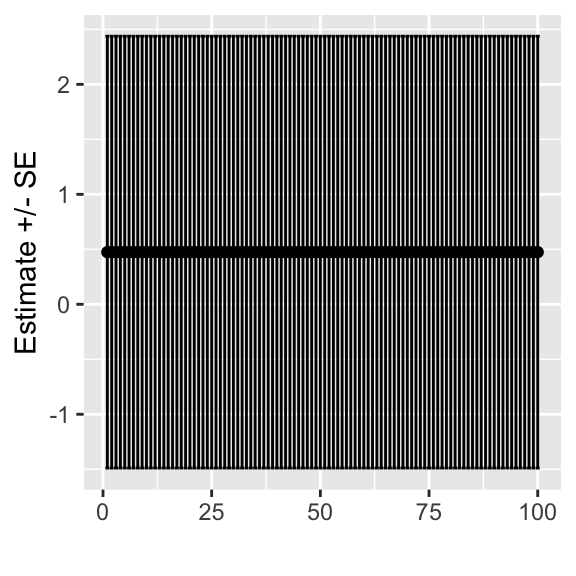
\includegraphics{lec_7_modelselection_files/figure-beamer/unnamed-chunk-18-1} \end{center}

\end{block}

\begin{block}{}

\begin{center}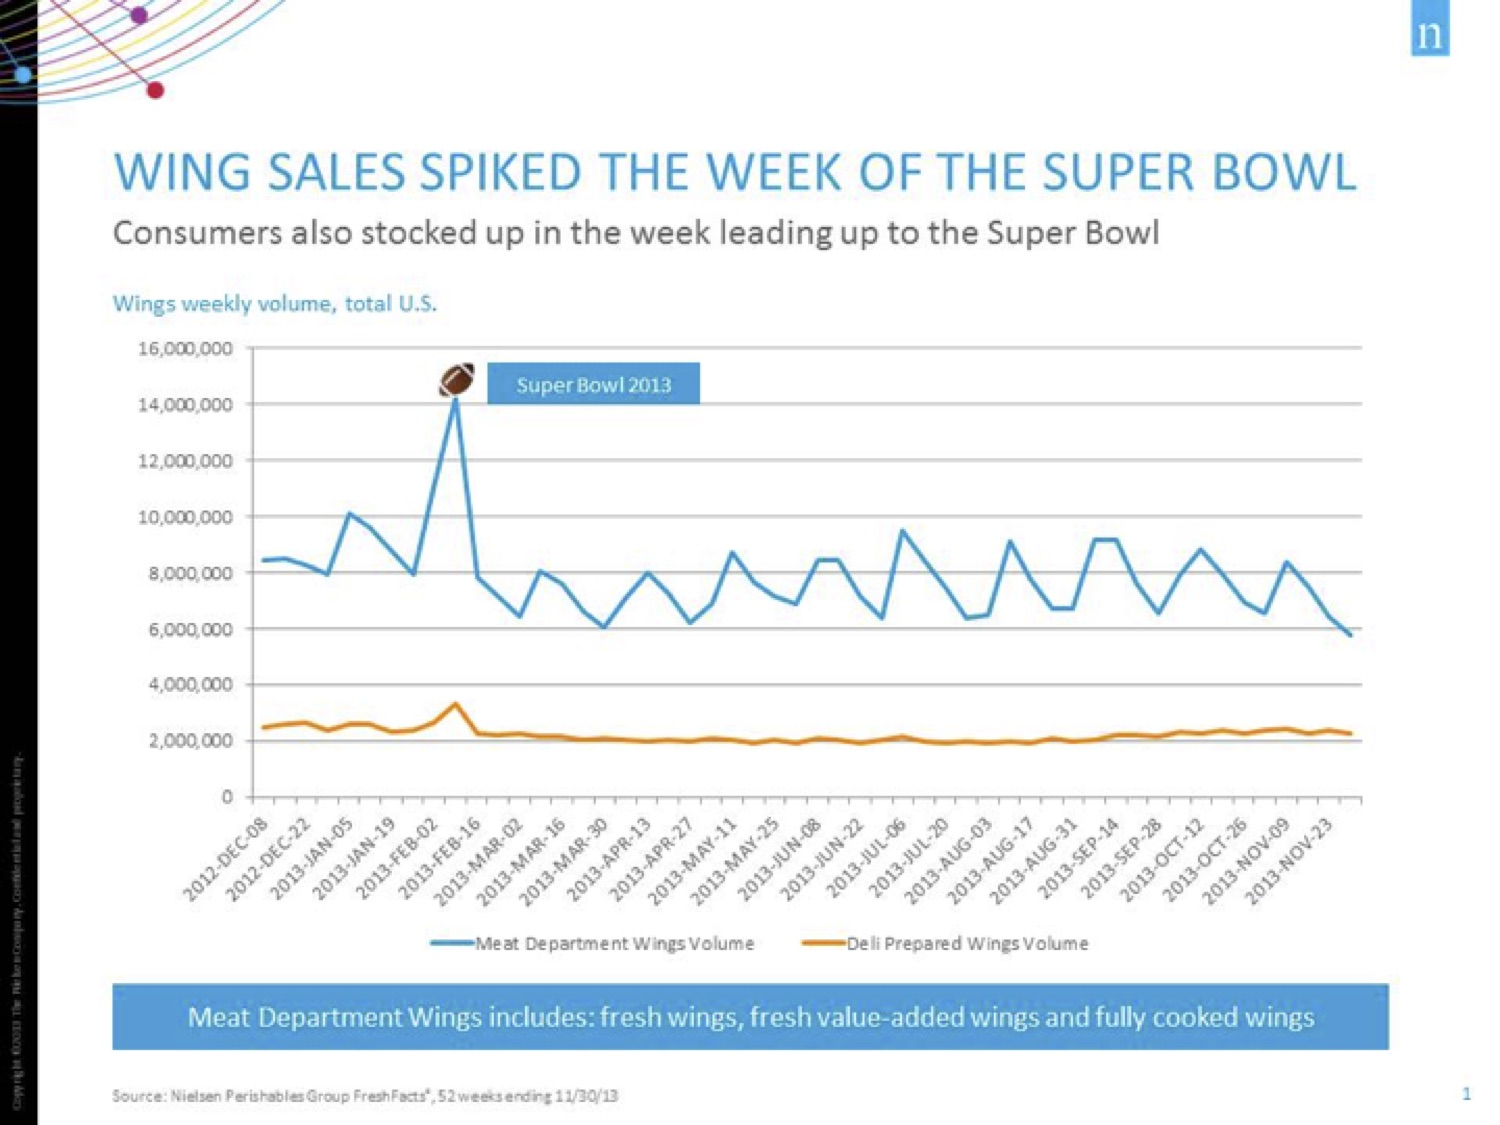
\includegraphics[width=800px]{wing_sales} \end{center}

\end{block}

\begin{block}{Percent Error Statistics}

Percent Error:

\[{ p }_{ t }=\frac { { e }_{ t }\cdot 100 }{ { Y }_{ t } }\]

Mean Absolute Percent Error (MAPE):

\[MAPE\quad =\quad E\left[ \left| { p }_{ t } \right|  \right]\] Root
Mean Square Percent Error (RMSPE):

\[RMSPE\quad =\quad \sqrt { E\left[ { p }_{ t }^{ 2 } \right]  }\]

\end{block}

\begin{block}{Issues with percent error statistics}

\begin{itemize}
\item
  What happens when Y = 0?
\item
  Distribution of percent errors tends to be highly skewed / long tails
\item
  MAPE tends to put higher penalty on positive errors
\item
  See Hyndman \& Koehler (2006)
\end{itemize}

\end{block}

\begin{block}{Scaled error statistics}

Define scaled error as

\[{ q }_{ t }=\frac { { e }_{ t } }{ \frac { 1 }{ n-1 } \sum _{ i=2 }^{ n }{ \left( { Y }_{ i }-{ Y }_{ i-1 } \right)  }  }\]

\begin{itemize}
\tightlist
\item
  denominator is MAE from random walk model, so performance is gauged
  relative to that
\item
  this does not allow for missing data
\end{itemize}

Absolute scaled error (ASE)

\[ASE=\left| { q }_{ t } \right|\] Mean absolute scaled error (MASE)

\[MASE=E\left[ \left| { q }_{ t } \right|  \right]\]

\end{block}

\begin{block}{Interpreting ASE and MASE}

All values are relative to the naïve random walk model

\begin{itemize}
\item
  Values \textless{} 1 indicate better performance than RW model
\item
  Values \textgreater{} 1 indicate worse performance than RW model
\end{itemize}

\end{block}

\begin{block}{Implementation in R}

\begin{itemize}
\tightlist
\item
  Fit an ARIMA model to `airmiles',holding out last 3 points
\end{itemize}

\begin{Shaded}
\begin{Highlighting}[]
\NormalTok{n =}\StringTok{ }\KeywordTok{length}\NormalTok{(airmiles)}
\NormalTok{air.model =}\StringTok{ }\KeywordTok{auto.arima}\NormalTok{(}\KeywordTok{log}\NormalTok{(airmiles[}\DecValTok{1}\OperatorTok{:}\NormalTok{(n}\DecValTok{-3}\NormalTok{)]))}
\end{Highlighting}
\end{Shaded}

\end{block}

\begin{block}{Implementation in R}

\begin{itemize}
\tightlist
\item
  Forecast the fitted model 3 steps ahead
\item
  Use holdout data to evaluate accuracy
\end{itemize}

\begin{Shaded}
\begin{Highlighting}[]
\NormalTok{air.forecast =}\StringTok{ }\KeywordTok{forecast}\NormalTok{(air.model, }\DataTypeTok{h =} \DecValTok{3}\NormalTok{)}
\KeywordTok{plot}\NormalTok{(air.forecast)}
\end{Highlighting}
\end{Shaded}

\begin{center}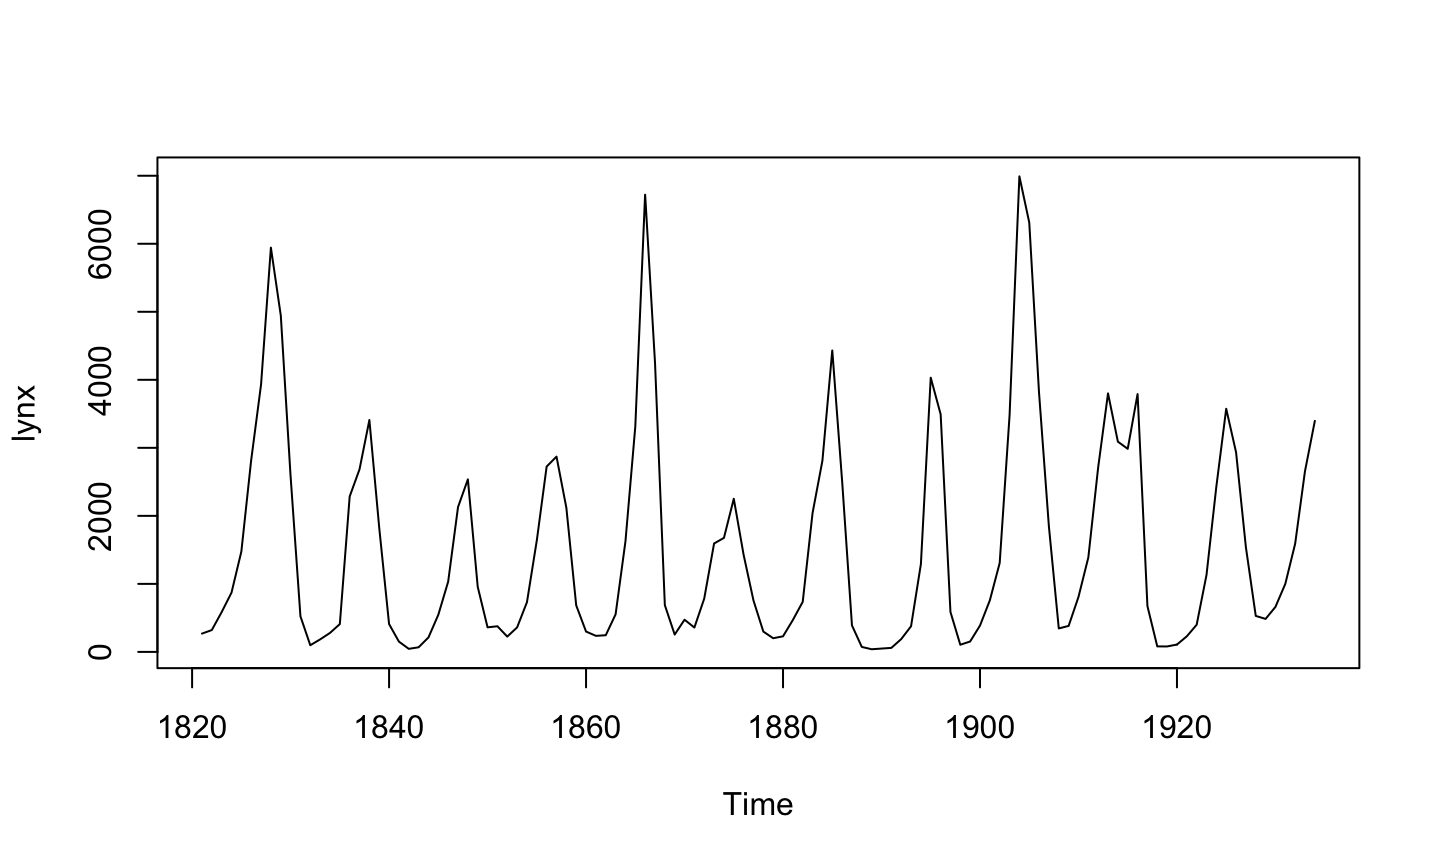
\includegraphics{lec_7_modelselection_files/figure-beamer/unnamed-chunk-21-1} \end{center}

\end{block}

\begin{block}{Implementation in R}

Evaluate RMSE / MASE statistics for 3 holdouts

\begin{Shaded}
\begin{Highlighting}[]
\KeywordTok{accuracy}\NormalTok{(air.forecast, }\KeywordTok{log}\NormalTok{(airmiles[(n}\DecValTok{-2}\NormalTok{)}\OperatorTok{:}\NormalTok{n]), }\DataTypeTok{test =} \DecValTok{3}\NormalTok{)}
\end{Highlighting}
\end{Shaded}

\begin{verbatim}
##                  ME      RMSE       MAE       MPE     MAPE     MASE
## Test set -0.4183656 0.4183656 0.4183656 -4.051598 4.051598 2.010664
\end{verbatim}

Evaluate RMSE / MASE statistics for only last holdout

\begin{Shaded}
\begin{Highlighting}[]
\KeywordTok{accuracy}\NormalTok{(air.forecast, }\KeywordTok{log}\NormalTok{(airmiles[(n}\DecValTok{-2}\NormalTok{)}\OperatorTok{:}\NormalTok{n]), }\DataTypeTok{test =} \DecValTok{1}\NormalTok{)}
\end{Highlighting}
\end{Shaded}

\begin{verbatim}
##                  ME      RMSE       MAE       MPE     MAPE     MASE
## Test set -0.1987598 0.1987598 0.1987598 -1.960106 1.960106 0.955239
\end{verbatim}

\end{block}

\end{frame}

\begin{frame}{Performance metrics summary}
\protect\hypertarget{performance-metrics-summary}{}

Raw statistics (e.g.~MSE, RMSE) shouldn't be applied for data of
different scale

Percent error metrics (e.g.~MAPE) may be skewed \& undefined for real
zeroes

Scaled error metrics (ASE, MASE) have been shown to be more robust
meta-analyses of many datasets + Hyndman \& Koehler (2006)

\begin{block}{Questions?}

\end{block}

\end{frame}

\end{document}
